\documentclass[1p]{elsarticle_modified}
%\bibliographystyle{elsarticle-num}

%\usepackage[colorlinks]{hyperref}
%\usepackage{abbrmath_seonhwa} %\Abb, \Ascr, \Acal ,\Abf, \Afrak
\usepackage{amsfonts}
\usepackage{amssymb}
\usepackage{amsmath}
\usepackage{amsthm}
\usepackage{scalefnt}
\usepackage{amsbsy}
\usepackage{kotex}
\usepackage{caption}
\usepackage{subfig}
\usepackage{color}
\usepackage{graphicx}
\usepackage{xcolor} %% white, black, red, green, blue, cyan, magenta, yellow
\usepackage{float}
\usepackage{setspace}
\usepackage{hyperref}

\usepackage{tikz}
\usetikzlibrary{arrows}

\usepackage{multirow}
\usepackage{array} % fixed length table
\usepackage{hhline}

%%%%%%%%%%%%%%%%%%%%%
\makeatletter
\renewcommand*\env@matrix[1][\arraystretch]{%
	\edef\arraystretch{#1}%
	\hskip -\arraycolsep
	\let\@ifnextchar\new@ifnextchar
	\array{*\c@MaxMatrixCols c}}
\makeatother %https://tex.stackexchange.com/questions/14071/how-can-i-increase-the-line-spacing-in-a-matrix
%%%%%%%%%%%%%%%

\usepackage[normalem]{ulem}

\newcommand{\msout}[1]{\ifmmode\text{\sout{\ensuremath{#1}}}\else\sout{#1}\fi}
%SOURCE: \msout is \stkout macro in https://tex.stackexchange.com/questions/20609/strikeout-in-math-mode

\newcommand{\cancel}[1]{
	\ifmmode
	{\color{red}\msout{#1}}
	\else
	{\color{red}\sout{#1}}
	\fi
}

\newcommand{\add}[1]{
	{\color{blue}\uwave{#1}}
}

\newcommand{\replace}[2]{
	\ifmmode
	{\color{red}\msout{#1}}{\color{blue}\uwave{#2}}
	\else
	{\color{red}\sout{#1}}{\color{blue}\uwave{#2}}
	\fi
}

\newcommand{\Sol}{\mathcal{S}} %segment
\newcommand{\D}{D} %diagram
\newcommand{\A}{\mathcal{A}} %arc


%%%%%%%%%%%%%%%%%%%%%%%%%%%%%5 test

\def\sl{\operatorname{\textup{SL}}(2,\Cbb)}
\def\psl{\operatorname{\textup{PSL}}(2,\Cbb)}
\def\quan{\mkern 1mu \triangleright \mkern 1mu}

\theoremstyle{definition}
\newtheorem{thm}{Theorem}[section]
\newtheorem{prop}[thm]{Proposition}
\newtheorem{lem}[thm]{Lemma}
\newtheorem{ques}[thm]{Question}
\newtheorem{cor}[thm]{Corollary}
\newtheorem{defn}[thm]{Definition}
\newtheorem{exam}[thm]{Example}
\newtheorem{rmk}[thm]{Remark}
\newtheorem{alg}[thm]{Algorithm}

\newcommand{\I}{\sqrt{-1}}
\begin{document}

%\begin{frontmatter}
%
%\title{Boundary parabolic representations of knots up to 8 crossings}
%
%%% Group authors per affiliation:
%\author{Yunhi Cho} 
%\address{Department of Mathematics, University of Seoul, Seoul, Korea}
%\ead{yhcho@uos.ac.kr}
%
%
%\author{Seonhwa Kim} %\fnref{s_kim}}
%\address{Center for Geometry and Physics, Institute for Basic Science, Pohang, 37673, Korea}
%\ead{ryeona17@ibs.re.kr}
%
%\author{Hyuk Kim}
%\address{Department of Mathematical Sciences, Seoul National University, Seoul 08826, Korea}
%\ead{hyukkim@snu.ac.kr}
%
%\author{Seokbeom Yoon}
%\address{Department of Mathematical Sciences, Seoul National University, Seoul, 08826,  Korea}
%\ead{sbyoon15@snu.ac.kr}
%
%\begin{abstract}
%We find all boundary parabolic representation of knots up to 8 crossings.
%
%\end{abstract}
%\begin{keyword}
%    \MSC[2010] 57M25 
%\end{keyword}
%
%\end{frontmatter}

%\linenumbers
%\tableofcontents
%
\newcommand\colored[1]{\textcolor{white}{\rule[-0.35ex]{0.8em}{1.4ex}}\kern-0.8em\color{red} #1}%
%\newcommand\colored[1]{\textcolor{white}{ #1}\kern-2.17ex	\textcolor{white}{ #1}\kern-1.81ex	\textcolor{white}{ #1}\kern-2.15ex\color{red}#1	}

{\Large $\underline{11n_{156}~(K11n_{156})}$}

\setlength{\tabcolsep}{10pt}
\renewcommand{\arraystretch}{1.6}
\vspace{1cm}\begin{tabular}{m{100pt}>{\centering\arraybackslash}m{274pt}}
\multirow{5}{120pt}{
	\centering
	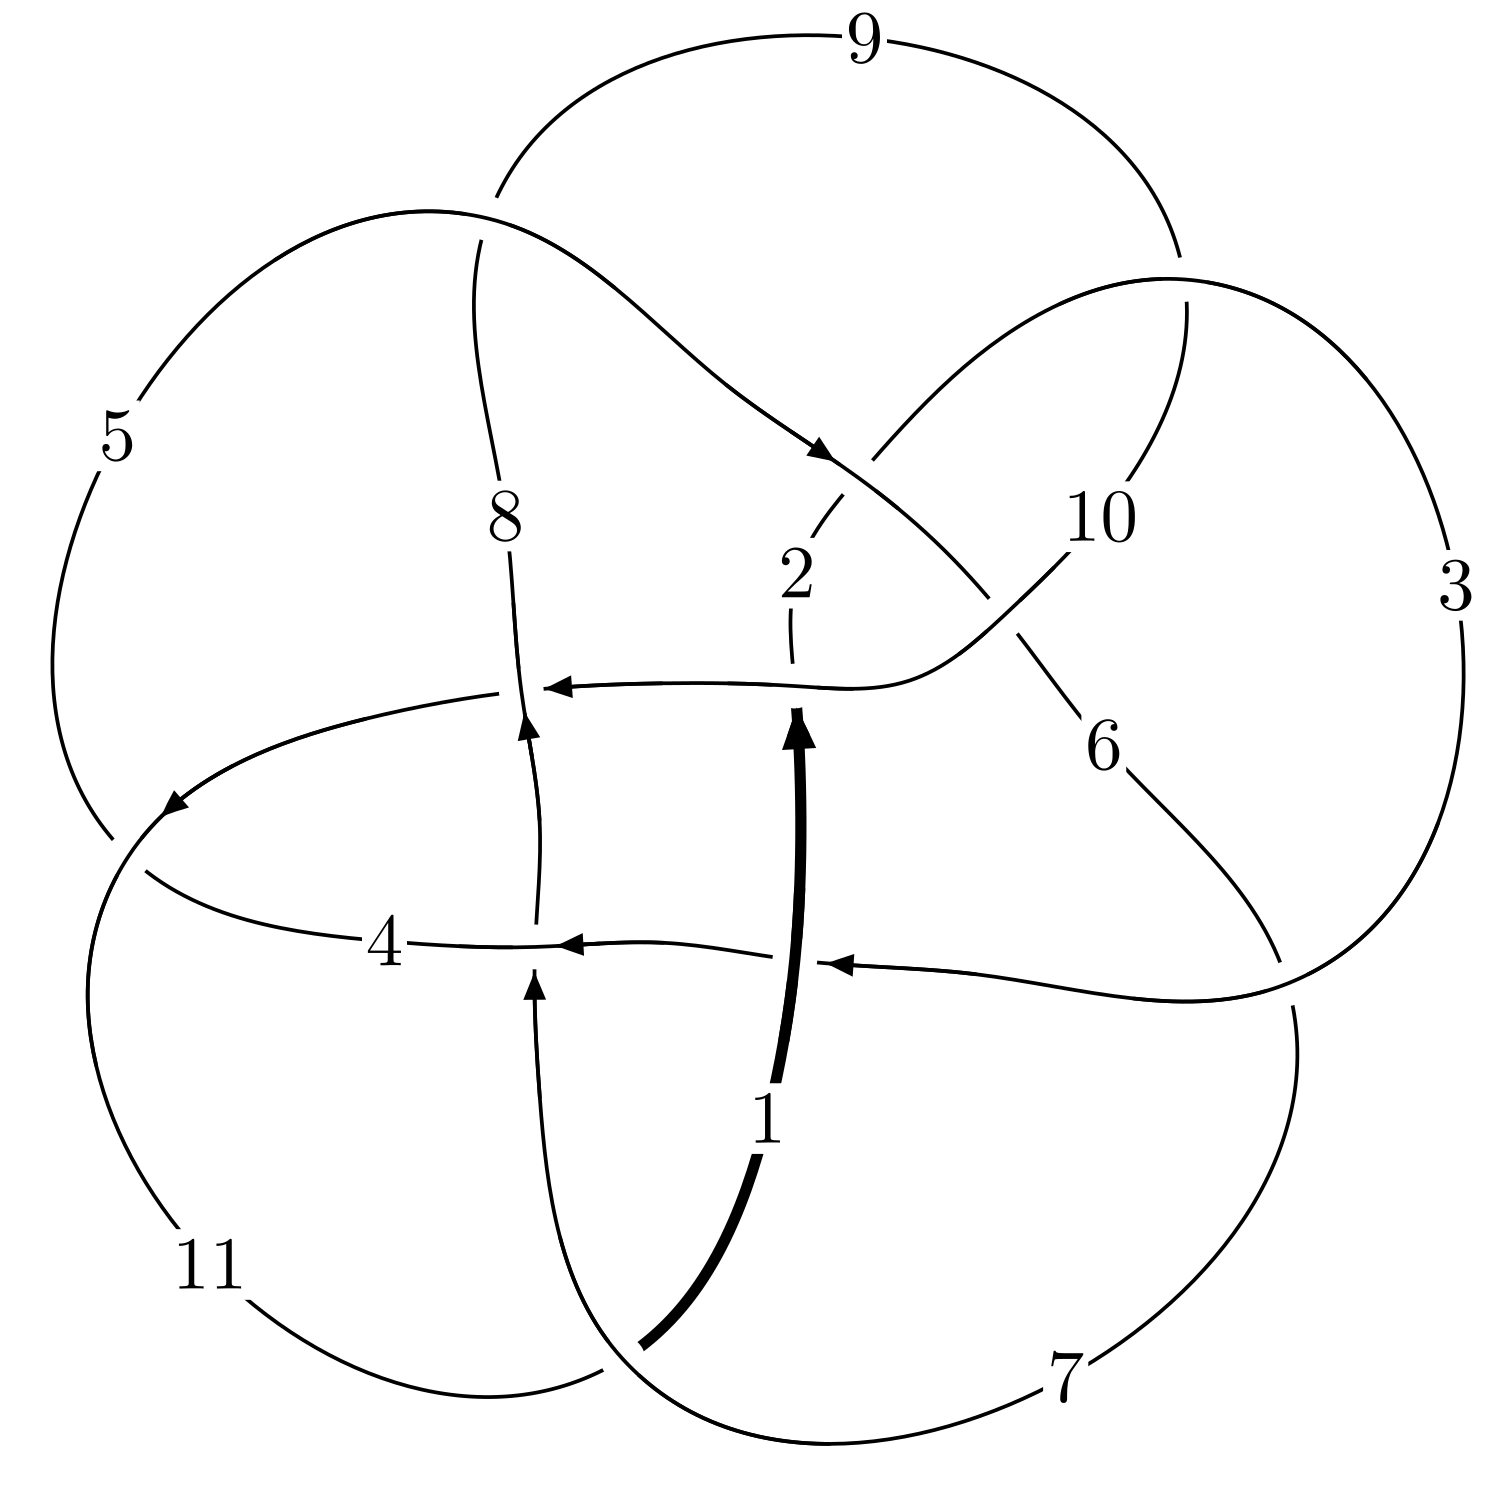
\includegraphics[width=112pt]{../../../GIT/diagram.site/Diagrams/png/772_11n_156.png}\\
\ \ \ A knot diagram\footnotemark}&
\allowdisplaybreaks
\textbf{Linearized knot diagam} \\
\cline{2-2}
 &
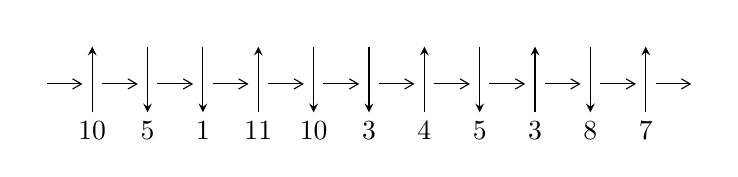
\begin{tikzpicture}[x=20pt, y=17pt]
	% nodes
	\node (C0) at (0, 0) {};
	\node (C1) at (1, 0) {};
	\node (C1U) at (1, +1) {};
	\node (C1D) at (1, -1) {10};

	\node (C2) at (2, 0) {};
	\node (C2U) at (2, +1) {};
	\node (C2D) at (2, -1) {5};

	\node (C3) at (3, 0) {};
	\node (C3U) at (3, +1) {};
	\node (C3D) at (3, -1) {1};

	\node (C4) at (4, 0) {};
	\node (C4U) at (4, +1) {};
	\node (C4D) at (4, -1) {11};

	\node (C5) at (5, 0) {};
	\node (C5U) at (5, +1) {};
	\node (C5D) at (5, -1) {10};

	\node (C6) at (6, 0) {};
	\node (C6U) at (6, +1) {};
	\node (C6D) at (6, -1) {3};

	\node (C7) at (7, 0) {};
	\node (C7U) at (7, +1) {};
	\node (C7D) at (7, -1) {4};

	\node (C8) at (8, 0) {};
	\node (C8U) at (8, +1) {};
	\node (C8D) at (8, -1) {5};

	\node (C9) at (9, 0) {};
	\node (C9U) at (9, +1) {};
	\node (C9D) at (9, -1) {3};

	\node (C10) at (10, 0) {};
	\node (C10U) at (10, +1) {};
	\node (C10D) at (10, -1) {8};

	\node (C11) at (11, 0) {};
	\node (C11U) at (11, +1) {};
	\node (C11D) at (11, -1) {7};
	\node (C12) at (12, 0) {};

	% arrows
	\draw[->,>={angle 60}]
	(C0) edge (C1) (C1) edge (C2) (C2) edge (C3) (C3) edge (C4) (C4) edge (C5) (C5) edge (C6) (C6) edge (C7) (C7) edge (C8) (C8) edge (C9) (C9) edge (C10) (C10) edge (C11) (C11) edge (C12) ;	\draw[->,>=stealth]
	(C1D) edge (C1U) (C2U) edge (C2D) (C3U) edge (C3D) (C4D) edge (C4U) (C5U) edge (C5D) (C6U) edge (C6D) (C7D) edge (C7U) (C8U) edge (C8D) (C9D) edge (C9U) (C10U) edge (C10D) (C11D) edge (C11U) ;
	\end{tikzpicture} \\
\hhline{~~} \\& 
\textbf{Solving Sequence} \\ \cline{2-2} 
 &
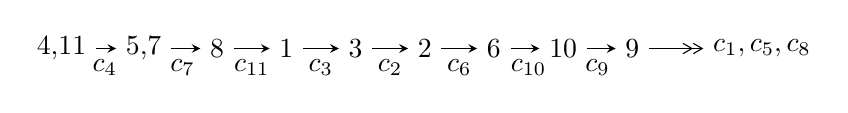
\begin{tikzpicture}[x=25pt, y=7pt]
	% node
	\node (A0) at (-1/8, 0) {4,11};
	\node (A1) at (17/16, 0) {5,7};
	\node (A2) at (17/8, 0) {8};
	\node (A3) at (25/8, 0) {1};
	\node (A4) at (33/8, 0) {3};
	\node (A5) at (41/8, 0) {2};
	\node (A6) at (49/8, 0) {6};
	\node (A7) at (57/8, 0) {10};
	\node (A8) at (65/8, 0) {9};
	\node (C1) at (1/2, -1) {$c_{4}$};
	\node (C2) at (13/8, -1) {$c_{7}$};
	\node (C3) at (21/8, -1) {$c_{11}$};
	\node (C4) at (29/8, -1) {$c_{3}$};
	\node (C5) at (37/8, -1) {$c_{2}$};
	\node (C6) at (45/8, -1) {$c_{6}$};
	\node (C7) at (53/8, -1) {$c_{10}$};
	\node (C8) at (61/8, -1) {$c_{9}$};
	\node (A9) at (10, 0) {$c_{1},c_{5},c_{8}$};

	% edge
	\draw[->,>=stealth]	
	(A0) edge (A1) (A1) edge (A2) (A2) edge (A3) (A3) edge (A4) (A4) edge (A5) (A5) edge (A6) (A6) edge (A7) (A7) edge (A8) ;
	\draw[->>,>={angle 60}]	
	(A8) edge (A9);
\end{tikzpicture} \\ 

\end{tabular} \\

\footnotetext{
The image of knot diagram is generated by the software ``\textbf{Draw programme}" developed by Andrew Bartholomew(\url{http://www.layer8.co.uk/maths/draw/index.htm\#Running-draw}), where we modified some parts for our purpose(\url{https://github.com/CATsTAILs/LinksPainter}).
}\phantom \\ \newline 
\centering \textbf{Ideals for irreducible components\footnotemark of $X_{\text{par}}$} 
 
\begin{align*}
I^u_{1}&=\langle 
286 u^{13}+1025 u^{12}+\cdots+189 b+494,\;a-1,\\
\phantom{I^u_{1}}&\phantom{= \langle  }2 u^{14}+3 u^{13}+6 u^{12}+u^{11}+11 u^{10}+5 u^9+20 u^8-2 u^7+15 u^6-5 u^5+11 u^4-7 u^3+7 u^2-3 u+1\rangle \\
I^u_{2}&=\langle 
2 u^7-14 u^6-8 u^5-21 u^4+25 u^3-19 u^2+9 b+30 u-14,\;a+1,\\
\phantom{I^u_{2}}&\phantom{= \langle  }2 u^8+2 u^6-5 u^5+4 u^4-6 u^3+5 u^2-2 u+1\rangle \\
I^u_{3}&=\langle 
-1.76422\times10^{54} u^{35}-3.41094\times10^{54} u^{34}+\cdots+1.61573\times10^{53} b+2.47914\times10^{53},\\
\phantom{I^u_{3}}&\phantom{= \langle  }3.12290\times10^{54} u^{35}+4.43281\times10^{54} u^{34}+\cdots+2.30819\times10^{52} a-3.74791\times10^{54},\;2 u^{36}+2 u^{35}+\cdots-14 u+1\rangle \\
I^u_{4}&=\langle 
4 u^3+6 u^2+3 b+4 u+1,\;4 u^3+12 u^2+3 a+10 u+1,\;2 u^4+4 u^3+2 u^2+1\rangle \\
\\
\end{align*}
\raggedright * 4 irreducible components of $\dim_{\mathbb{C}}=0$, with total 62 representations.\\
\footnotetext{All coefficients of polynomials are rational numbers. But the coefficients are sometimes approximated in decimal forms when there is not enough margin.}
\newpage
\renewcommand{\arraystretch}{1}
\centering \section*{I. $I^u_{1}= \langle 286 u^{13}+1025 u^{12}+\cdots+189 b+494,\;a-1,\;2 u^{14}+3 u^{13}+\cdots-3 u+1 \rangle$}
\flushleft \textbf{(i) Arc colorings}\\
\begin{tabular}{m{7pt} m{180pt} m{7pt} m{180pt} }
\flushright $a_{4}=$&$\begin{pmatrix}1\\0\end{pmatrix}$ \\
\flushright $a_{11}=$&$\begin{pmatrix}0\\u\end{pmatrix}$ \\
\flushright $a_{5}=$&$\begin{pmatrix}1\\- u^2\end{pmatrix}$ \\
\flushright $a_{7}=$&$\begin{pmatrix}1\\-1.51323 u^{13}-5.42328 u^{12}+\cdots-0.164021 u-2.61376\end{pmatrix}$ \\
\flushright $a_{8}=$&$\begin{pmatrix}-1.51323 u^{13}-5.42328 u^{12}+\cdots-0.164021 u-1.61376\\-1.51323 u^{13}-5.42328 u^{12}+\cdots-0.164021 u-2.61376\end{pmatrix}$ \\
\flushright $a_{1}=$&$\begin{pmatrix}u\\-3.15344 u^{13}-6.81481 u^{12}+\cdots-3.88360 u+0.756614\end{pmatrix}$ \\
\flushright $a_{3}=$&$\begin{pmatrix}2.08466 u^{13}+3.32804 u^{12}+\cdots+3.97354 u-0.576720\\2.06349 u^{13}+2.26984 u^{12}+\cdots+5.63492 u-2.73016\end{pmatrix}$ \\
\flushright $a_{2}=$&$\begin{pmatrix}3.56614 u^{13}+4.35450 u^{12}+\cdots+8.86772 u-3.40741\\3.43915 u^{13}+4.67196 u^{12}+\cdots+8.16931 u-3.32804\end{pmatrix}$ \\
\flushright $a_{6}=$&$\begin{pmatrix}-4.79365 u^{13}-11.9206 u^{12}+\cdots-4.74603 u-0.777778\\-5.22751 u^{13}-10.4550 u^{12}+\cdots-8.65608 u+1.37037\end{pmatrix}$ \\
\flushright $a_{10}=$&$\begin{pmatrix}-5.46032 u^{13}-10.2540 u^{12}+\cdots-9.41270 u+2.55556\\-2.30688 u^{13}-3.43915 u^{12}+\cdots-4.52910 u+1.79894\end{pmatrix}$ \\
\flushright $a_{9}=$&$\begin{pmatrix}2.08466 u^{13}+3.32804 u^{12}+\cdots+3.97354 u-0.576720\\-3.01587 u^{13}-7.50794 u^{12}+\cdots-3.39683 u-0.936508\end{pmatrix}$\\ \flushright $a_{9}=$&$\begin{pmatrix}2.08466 u^{13}+3.32804 u^{12}+\cdots+3.97354 u-0.576720\\-3.01587 u^{13}-7.50794 u^{12}+\cdots-3.39683 u-0.936508\end{pmatrix}$\\&\end{tabular}
\flushleft \textbf{(ii) Obstruction class $= -1$}\\~\\
\flushleft \textbf{(iii) Cusp Shapes $= -\frac{136}{27} u^{13}-\frac{1550}{189} u^{12}-\frac{2491}{189} u^{11}+\frac{248}{189} u^{10}-\frac{1103}{63} u^9-\frac{2428}{189} u^8-\frac{2563}{63} u^7+\frac{1360}{189} u^6-\frac{1738}{189} u^5+\frac{1937}{189} u^4-\frac{1363}{63} u^3-\frac{16}{27} u^2-\frac{2242}{189} u-\frac{176}{189}$}\\~\\
\newpage\renewcommand{\arraystretch}{1}
\flushleft \textbf{(iv) u-Polynomials at the component}\newline \\
\begin{tabular}{m{50pt}|m{274pt}}
Crossings & \hspace{64pt}u-Polynomials at each crossing \\
\hline $$\begin{aligned}c_{1}\end{aligned}$$&$\begin{aligned}
&4(4 u^{14}+43 u^{13}+\cdots+336 u+64)
\end{aligned}$\\
\hline $$\begin{aligned}c_{2},c_{5}\end{aligned}$$&$\begin{aligned}
&2(2 u^{14}- u^{13}+\cdots+9 u^2+1)
\end{aligned}$\\
\hline $$\begin{aligned}c_{3},c_{10}\end{aligned}$$&$\begin{aligned}
&u^{14}-2 u^{13}+\cdots-3 u+2
\end{aligned}$\\
\hline $$\begin{aligned}c_{4},c_{11}\end{aligned}$$&$\begin{aligned}
&2(2 u^{14}-3 u^{13}+\cdots+3 u+1)
\end{aligned}$\\
\hline $$\begin{aligned}c_{6},c_{8}\end{aligned}$$&$\begin{aligned}
&u^{14}- u^{13}+\cdots-13 u+2
\end{aligned}$\\
\hline $$\begin{aligned}c_{7}\end{aligned}$$&$\begin{aligned}
&u^{14}-9 u^{13}+\cdots-24 u+8
\end{aligned}$\\
\hline $$\begin{aligned}c_{9}\end{aligned}$$&$\begin{aligned}
&u^{14}-10 u^{13}+\cdots-80 u+32
\end{aligned}$\\
\hline
\end{tabular}\\~\\
\newpage\renewcommand{\arraystretch}{1}
\flushleft \textbf{(v) Riley Polynomials at the component}\newline \\
\begin{tabular}{m{50pt}|m{274pt}}
Crossings & \hspace{64pt}Riley Polynomials at each crossing \\
\hline $$\begin{aligned}c_{1}\end{aligned}$$&$\begin{aligned}
&16(16 y^{14}-105 y^{13}+\cdots+16128 y+4096)
\end{aligned}$\\
\hline $$\begin{aligned}c_{2},c_{5}\end{aligned}$$&$\begin{aligned}
&4(4 y^{14}+83 y^{13}+\cdots+18 y+1)
\end{aligned}$\\
\hline $$\begin{aligned}c_{3},c_{10}\end{aligned}$$&$\begin{aligned}
&y^{14}+4 y^{13}+\cdots-5 y+4
\end{aligned}$\\
\hline $$\begin{aligned}c_{4},c_{11}\end{aligned}$$&$\begin{aligned}
&4(4 y^{14}+15 y^{13}+\cdots+5 y+1)
\end{aligned}$\\
\hline $$\begin{aligned}c_{6},c_{8}\end{aligned}$$&$\begin{aligned}
&y^{14}+7 y^{13}+\cdots-33 y+4
\end{aligned}$\\
\hline $$\begin{aligned}c_{7}\end{aligned}$$&$\begin{aligned}
&y^{14}+3 y^{13}+\cdots-96 y+64
\end{aligned}$\\
\hline $$\begin{aligned}c_{9}\end{aligned}$$&$\begin{aligned}
&y^{14}-10 y^{13}+\cdots+5376 y+1024
\end{aligned}$\\
\hline
\end{tabular}\\~\\
\newpage\flushleft \textbf{(vi) Complex Volumes and Cusp Shapes}
$$\begin{array}{c|c|c}  
\text{Solutions to }I^u_{1}& \I (\text{vol} + \sqrt{-1}CS) & \text{Cusp shape}\\
 \hline 
\begin{aligned}
u &= -0.747471 + 0.736656 I \\
a &= \phantom{-}1.00000\phantom{ +0.000000I} \\
b &= -1.190140 + 0.650810 I\end{aligned}
 & \phantom{-}2.08139 - 2.02696 I & \phantom{-}1.83038 + 2.57438 I \\ \hline\begin{aligned}
u &= -0.747471 - 0.736656 I \\
a &= \phantom{-}1.00000\phantom{ +0.000000I} \\
b &= -1.190140 - 0.650810 I\end{aligned}
 & \phantom{-}2.08139 + 2.02696 I & \phantom{-}1.83038 - 2.57438 I \\ \hline\begin{aligned}
u &= \phantom{-}0.068372 + 0.773508 I \\
a &= \phantom{-}1.00000\phantom{ +0.000000I} \\
b &= \phantom{-}0.483737 - 0.312119 I\end{aligned}
 & \phantom{-}0.50090 - 2.66807 I & \phantom{-}3.96052 + 3.99756 I \\ \hline\begin{aligned}
u &= \phantom{-}0.068372 - 0.773508 I \\
a &= \phantom{-}1.00000\phantom{ +0.000000I} \\
b &= \phantom{-}0.483737 + 0.312119 I\end{aligned}
 & \phantom{-}0.50090 + 2.66807 I & \phantom{-}3.96052 - 3.99756 I \\ \hline\begin{aligned}
u &= \phantom{-}0.863068 + 0.906873 I \\
a &= \phantom{-}1.00000\phantom{ +0.000000I} \\
b &= -1.23002 - 1.06519 I\end{aligned}
 & \phantom{-}1.01240 + 7.85357 I & \phantom{-}1.37704 - 6.81636 I \\ \hline\begin{aligned}
u &= \phantom{-}0.863068 - 0.906873 I \\
a &= \phantom{-}1.00000\phantom{ +0.000000I} \\
b &= -1.23002 + 1.06519 I\end{aligned}
 & \phantom{-}1.01240 - 7.85357 I & \phantom{-}1.37704 + 6.81636 I \\ \hline\begin{aligned}
u &= -0.606706 + 1.104340 I \\
a &= \phantom{-}1.00000\phantom{ +0.000000I} \\
b &= -0.474186 + 0.465380 I\end{aligned}
 & \phantom{-}2.86726 - 1.52978 I & -3.12219 + 1.19653 I \\ \hline\begin{aligned}
u &= -0.606706 - 1.104340 I \\
a &= \phantom{-}1.00000\phantom{ +0.000000I} \\
b &= -0.474186 - 0.465380 I\end{aligned}
 & \phantom{-}2.86726 + 1.52978 I & -3.12219 - 1.19653 I \\ \hline\begin{aligned}
u &= \phantom{-}0.376941 + 0.517480 I \\
a &= \phantom{-}1.00000\phantom{ +0.000000I} \\
b &= -0.75145 + 1.71976 I\end{aligned}
 & \phantom{-}6.55927 + 6.69837 I & -2.55381 - 9.47495 I \\ \hline\begin{aligned}
u &= \phantom{-}0.376941 - 0.517480 I \\
a &= \phantom{-}1.00000\phantom{ +0.000000I} \\
b &= -0.75145 - 1.71976 I\end{aligned}
 & \phantom{-}6.55927 - 6.69837 I & -2.55381 + 9.47495 I\\
 \hline 
 \end{array}$$\newpage$$\begin{array}{c|c|c}  
\text{Solutions to }I^u_{1}& \I (\text{vol} + \sqrt{-1}CS) & \text{Cusp shape}\\
 \hline 
\begin{aligned}
u &= \phantom{-}0.387427 + 0.358801 I \\
a &= \phantom{-}1.00000\phantom{ +0.000000I} \\
b &= -0.081855 - 1.118280 I\end{aligned}
 & -1.68063 + 1.15707 I & -4.41586 - 6.34189 I \\ \hline\begin{aligned}
u &= \phantom{-}0.387427 - 0.358801 I \\
a &= \phantom{-}1.00000\phantom{ +0.000000I} \\
b &= -0.081855 + 1.118280 I\end{aligned}
 & -1.68063 - 1.15707 I & -4.41586 + 6.34189 I \\ \hline\begin{aligned}
u &= -1.09163 + 1.20653 I \\
a &= \phantom{-}1.00000\phantom{ +0.000000I} \\
b &= -1.25608 + 0.97829 I\end{aligned}
 & \phantom{-}8.3986 - 15.3972 I & \phantom{-}1.29891 + 7.67212 I \\ \hline\begin{aligned}
u &= -1.09163 - 1.20653 I \\
a &= \phantom{-}1.00000\phantom{ +0.000000I} \\
b &= -1.25608 - 0.97829 I\end{aligned}
 & \phantom{-}8.3986 + 15.3972 I & \phantom{-}1.29891 - 7.67212 I\\
 \hline 
 \end{array}$$\newpage\newpage\renewcommand{\arraystretch}{1}
\centering \section*{II. $I^u_{2}= \langle 2 u^7-14 u^6+\cdots+9 b-14,\;a+1,\;2 u^8+2 u^6-5 u^5+4 u^4-6 u^3+5 u^2-2 u+1 \rangle$}
\flushleft \textbf{(i) Arc colorings}\\
\begin{tabular}{m{7pt} m{180pt} m{7pt} m{180pt} }
\flushright $a_{4}=$&$\begin{pmatrix}1\\0\end{pmatrix}$ \\
\flushright $a_{11}=$&$\begin{pmatrix}0\\u\end{pmatrix}$ \\
\flushright $a_{5}=$&$\begin{pmatrix}1\\- u^2\end{pmatrix}$ \\
\flushright $a_{7}=$&$\begin{pmatrix}-1\\-\frac{2}{9} u^7+\frac{14}{9} u^6+\cdots-\frac{10}{3} u+\frac{14}{9}\end{pmatrix}$ \\
\flushright $a_{8}=$&$\begin{pmatrix}-\frac{2}{9} u^7+\frac{14}{9} u^6+\cdots-\frac{10}{3} u+\frac{5}{9}\\-\frac{2}{9} u^7+\frac{14}{9} u^6+\cdots-\frac{10}{3} u+\frac{14}{9}\end{pmatrix}$ \\
\flushright $a_{1}=$&$\begin{pmatrix}u\\-\frac{14}{9} u^7-\frac{10}{9} u^6+\cdots-\frac{1}{3} u-\frac{1}{9}\end{pmatrix}$ \\
\flushright $a_{3}=$&$\begin{pmatrix}\frac{10}{9} u^7+\frac{2}{9} u^6+\cdots+\frac{5}{3} u+\frac{2}{9}\\\frac{2}{3} u^7+2 u^5+\cdots+\frac{5}{3} u-\frac{4}{3}\end{pmatrix}$ \\
\flushright $a_{2}=$&$\begin{pmatrix}\frac{20}{9} u^7+\frac{10}{9} u^6+\cdots+3 u-\frac{11}{9}\\-\frac{4}{9} u^7-\frac{8}{9} u^6+\cdots+\frac{4}{3} u-\frac{8}{9}\end{pmatrix}$ \\
\flushright $a_{6}=$&$\begin{pmatrix}\frac{2}{3} u^6+\frac{2}{3} u^5+\cdots-\frac{4}{3} u+\frac{1}{3}\\\frac{2}{3} u^6+\frac{2}{3} u^5+\cdots-\frac{4}{3} u+\frac{1}{3}\end{pmatrix}$ \\
\flushright $a_{10}=$&$\begin{pmatrix}-\frac{8}{3} u^7-\frac{2}{3} u^6+\cdots-\frac{10}{3} u+1\\-\frac{10}{9} u^7+\frac{4}{9} u^6+\cdots-2 u+\frac{10}{9}\end{pmatrix}$ \\
\flushright $a_{9}=$&$\begin{pmatrix}-\frac{10}{9} u^7-\frac{2}{9} u^6+\cdots-\frac{5}{3} u-\frac{2}{9}\\\frac{4}{3} u^7+\frac{8}{3} u^6+\cdots-2 u+\frac{2}{3}\end{pmatrix}$\\ \flushright $a_{9}=$&$\begin{pmatrix}-\frac{10}{9} u^7-\frac{2}{9} u^6+\cdots-\frac{5}{3} u-\frac{2}{9}\\\frac{4}{3} u^7+\frac{8}{3} u^6+\cdots-2 u+\frac{2}{3}\end{pmatrix}$\\&\end{tabular}
\flushleft \textbf{(ii) Obstruction class $= 1$}\\~\\
\flushleft \textbf{(iii) Cusp Shapes $= -\frac{166}{9} u^7-\frac{92}{9} u^6-\frac{194}{9} u^5+\frac{103}{3} u^4-\frac{128}{9} u^3+\frac{344}{9} u^2-18 u-\frac{59}{9}$}\\~\\
\newpage\renewcommand{\arraystretch}{1}
\flushleft \textbf{(iv) u-Polynomials at the component}\newline \\
\begin{tabular}{m{50pt}|m{274pt}}
Crossings & \hspace{64pt}u-Polynomials at each crossing \\
\hline $$\begin{aligned}c_{1}\end{aligned}$$&$\begin{aligned}
&4(4 u^8-8 u^7+17 u^5-13 u^4-2 u^3+13 u^2-3 u+1)
\end{aligned}$\\
\hline $$\begin{aligned}c_{2},c_{5}\end{aligned}$$&$\begin{aligned}
&2(2 u^8-2 u^7+4 u^6+u^5-11 u^4+5 u^3+6 u^2-5 u+1)
\end{aligned}$\\
\hline $$\begin{aligned}c_{3},c_{10}\end{aligned}$$&$\begin{aligned}
&u^8+2 u^7+3 u^6+2 u^5+2 u^4+3 u^3+6 u^2+6 u+2
\end{aligned}$\\
\hline $$\begin{aligned}c_{4},c_{11}\end{aligned}$$&$\begin{aligned}
&2(2 u^8+2 u^6-5 u^5+4 u^4-6 u^3+5 u^2-2 u+1)
\end{aligned}$\\
\hline $$\begin{aligned}c_{6},c_{8}\end{aligned}$$&$\begin{aligned}
&u^8+u^7+u^6+4 u^5+7 u^4- u^3-2 u^2+8 u+6
\end{aligned}$\\
\hline $$\begin{aligned}c_{7}\end{aligned}$$&$\begin{aligned}
&u^8+4 u^7+9 u^6+11 u^5+9 u^4+3 u^3-2 u+1
\end{aligned}$\\
\hline $$\begin{aligned}c_{9}\end{aligned}$$&$\begin{aligned}
&u^8- u^7-3 u^6-2 u^5+5 u^4+6 u^3+4 u^2+u+1
\end{aligned}$\\
\hline
\end{tabular}\\~\\
\newpage\renewcommand{\arraystretch}{1}
\flushleft \textbf{(v) Riley Polynomials at the component}\newline \\
\begin{tabular}{m{50pt}|m{274pt}}
Crossings & \hspace{64pt}Riley Polynomials at each crossing \\
\hline $$\begin{aligned}c_{1}\end{aligned}$$&$\begin{aligned}
&16\\
&\cdot(16 y^8-64 y^7+168 y^6-217 y^5+197 y^4-240 y^3+131 y^2+17 y+1)
\end{aligned}$\\
\hline $$\begin{aligned}c_{2},c_{5}\end{aligned}$$&$\begin{aligned}
&4(4 y^8+12 y^7-24 y^6-45 y^5+143 y^4-139 y^3+64 y^2-13 y+1)
\end{aligned}$\\
\hline $$\begin{aligned}c_{3},c_{10}\end{aligned}$$&$\begin{aligned}
&y^8+2 y^7+5 y^6+8 y^5+8 y^4+3 y^3+8 y^2-12 y+4
\end{aligned}$\\
\hline $$\begin{aligned}c_{4},c_{11}\end{aligned}$$&$\begin{aligned}
&4(4 y^8+8 y^7+20 y^6+11 y^5-20 y^4-12 y^3+9 y^2+6 y+1)
\end{aligned}$\\
\hline $$\begin{aligned}c_{6},c_{8}\end{aligned}$$&$\begin{aligned}
&y^8+y^7+7 y^6-4 y^5+49 y^4-81 y^3+104 y^2-88 y+36
\end{aligned}$\\
\hline $$\begin{aligned}c_{7}\end{aligned}$$&$\begin{aligned}
&y^8+2 y^7+11 y^6+17 y^5+33 y^4+53 y^3+30 y^2-4 y+1
\end{aligned}$\\
\hline $$\begin{aligned}c_{9}\end{aligned}$$&$\begin{aligned}
&y^8-7 y^7+15 y^6-14 y^5+29 y^4+2 y^3+14 y^2+7 y+1
\end{aligned}$\\
\hline
\end{tabular}\\~\\
\newpage\flushleft \textbf{(vi) Complex Volumes and Cusp Shapes}
$$\begin{array}{c|c|c}  
\text{Solutions to }I^u_{2}& \I (\text{vol} + \sqrt{-1}CS) & \text{Cusp shape}\\
 \hline 
\begin{aligned}
u &= -0.081144 + 0.964537 I \\
a &= -1.00000\phantom{ +0.000000I} \\
b &= -0.344131 - 0.211497 I\end{aligned}
 & -0.11790 + 2.52032 I & -8.47313 - 1.37245 I \\ \hline\begin{aligned}
u &= -0.081144 - 0.964537 I \\
a &= -1.00000\phantom{ +0.000000I} \\
b &= -0.344131 + 0.211497 I\end{aligned}
 & -0.11790 - 2.52032 I & -8.47313 + 1.37245 I \\ \hline\begin{aligned}
u &= \phantom{-}0.876567 + 0.170950 I \\
a &= -1.00000\phantom{ +0.000000I} \\
b &= \phantom{-}0.186359 + 1.054490 I\end{aligned}
 & \phantom{-}7.53561 + 5.92481 I & \phantom{-}2.17560 - 4.89559 I \\ \hline\begin{aligned}
u &= \phantom{-}0.876567 - 0.170950 I \\
a &= -1.00000\phantom{ +0.000000I} \\
b &= \phantom{-}0.186359 - 1.054490 I\end{aligned}
 & \phantom{-}7.53561 - 5.92481 I & \phantom{-}2.17560 + 4.89559 I \\ \hline\begin{aligned}
u &= \phantom{-}0.120498 + 0.535479 I \\
a &= -1.00000\phantom{ +0.000000I} \\
b &= \phantom{-}1.02903 - 1.25354 I\end{aligned}
 & -2.49208 + 1.02158 I & -16.3238 - 6.0123 I \\ \hline\begin{aligned}
u &= \phantom{-}0.120498 - 0.535479 I \\
a &= -1.00000\phantom{ +0.000000I} \\
b &= \phantom{-}1.02903 + 1.25354 I\end{aligned}
 & -2.49208 - 1.02158 I & -16.3238 + 6.0123 I \\ \hline\begin{aligned}
u &= -0.91592 + 1.17562 I \\
a &= -1.00000\phantom{ +0.000000I} \\
b &= \phantom{-}1.12874 - 0.87067 I\end{aligned}
 & -1.63576 - 8.28057 I & -4.87863 + 7.63527 I \\ \hline\begin{aligned}
u &= -0.91592 - 1.17562 I \\
a &= -1.00000\phantom{ +0.000000I} \\
b &= \phantom{-}1.12874 + 0.87067 I\end{aligned}
 & -1.63576 + 8.28057 I & -4.87863 - 7.63527 I\\
 \hline 
 \end{array}$$\newpage\newpage\renewcommand{\arraystretch}{1}
\centering \section*{III. $I^u_{3}= \langle -1.76\times10^{54} u^{35}-3.41\times10^{54} u^{34}+\cdots+1.62\times10^{53} b+2.48\times10^{53},\;3.12\times10^{54} u^{35}+4.43\times10^{54} u^{34}+\cdots+2.31\times10^{52} a-3.75\times10^{54},\;2 u^{36}+2 u^{35}+\cdots-14 u+1 \rangle$}
\flushleft \textbf{(i) Arc colorings}\\
\begin{tabular}{m{7pt} m{180pt} m{7pt} m{180pt} }
\flushright $a_{4}=$&$\begin{pmatrix}1\\0\end{pmatrix}$ \\
\flushright $a_{11}=$&$\begin{pmatrix}0\\u\end{pmatrix}$ \\
\flushright $a_{5}=$&$\begin{pmatrix}1\\- u^2\end{pmatrix}$ \\
\flushright $a_{7}=$&$\begin{pmatrix}-135.297 u^{35}-192.047 u^{34}+\cdots-1894.64 u+162.375\\10.9190 u^{35}+21.1108 u^{34}+\cdots+23.6339 u-1.53438\end{pmatrix}$ \\
\flushright $a_{8}=$&$\begin{pmatrix}-124.378 u^{35}-170.936 u^{34}+\cdots-1871.00 u+160.840\\10.9190 u^{35}+21.1108 u^{34}+\cdots+23.6339 u-1.53438\end{pmatrix}$ \\
\flushright $a_{1}=$&$\begin{pmatrix}140.578 u^{35}+183.175 u^{34}+\cdots+2437.80 u-225.735\\-22.7951 u^{35}-26.5223 u^{34}+\cdots-458.196 u+42.0517\end{pmatrix}$ \\
\flushright $a_{3}=$&$\begin{pmatrix}-203.081 u^{35}-272.115 u^{34}+\cdots-3148.94 u+274.459\\46.8092 u^{35}+61.5248 u^{34}+\cdots+699.352 u-58.6705\end{pmatrix}$ \\
\flushright $a_{2}=$&$\begin{pmatrix}-177.136 u^{35}-236.734 u^{34}+\cdots-2831.29 u+250.306\\44.3327 u^{35}+58.6254 u^{34}+\cdots+646.276 u-53.9528\end{pmatrix}$ \\
\flushright $a_{6}=$&$\begin{pmatrix}28.2278 u^{35}+40.0599 u^{34}+\cdots+373.025 u-32.8519\\-6.91942 u^{35}-4.84581 u^{34}+\cdots-223.697 u+19.9655\end{pmatrix}$ \\
\flushright $a_{10}=$&$\begin{pmatrix}104.432 u^{35}+141.715 u^{34}+\cdots+1653.06 u-152.962\\-13.3506 u^{35}-14.9377 u^{34}+\cdots-324.539 u+30.7209\end{pmatrix}$ \\
\flushright $a_{9}=$&$\begin{pmatrix}-117.271 u^{35}-167.192 u^{34}+\cdots-1630.91 u+139.095\\14.3939 u^{35}+26.3816 u^{34}+\cdots+50.7212 u-3.21539\end{pmatrix}$\\ \flushright $a_{9}=$&$\begin{pmatrix}-117.271 u^{35}-167.192 u^{34}+\cdots-1630.91 u+139.095\\14.3939 u^{35}+26.3816 u^{34}+\cdots+50.7212 u-3.21539\end{pmatrix}$\\&\end{tabular}
\flushleft \textbf{(ii) Obstruction class $= -1$}\\~\\
\flushleft \textbf{(iii) Cusp Shapes $= -284.262 u^{35}-374.406 u^{34}+\cdots-4742.13 u+418.350$}\\~\\
\newpage\renewcommand{\arraystretch}{1}
\flushleft \textbf{(iv) u-Polynomials at the component}\newline \\
\begin{tabular}{m{50pt}|m{274pt}}
Crossings & \hspace{64pt}u-Polynomials at each crossing \\
\hline $$\begin{aligned}c_{1}\end{aligned}$$&$\begin{aligned}
&4(2 u^{18}-16 u^{17}+\cdots-7 u+7)^{2}
\end{aligned}$\\
\hline $$\begin{aligned}c_{2},c_{5}\end{aligned}$$&$\begin{aligned}
&2(2 u^{36}+2 u^{35}+\cdots+1164 u+139)
\end{aligned}$\\
\hline $$\begin{aligned}c_{3},c_{10}\end{aligned}$$&$\begin{aligned}
&u^{36}-5 u^{35}+\cdots-20 u+2
\end{aligned}$\\
\hline $$\begin{aligned}c_{4},c_{11}\end{aligned}$$&$\begin{aligned}
&2(2 u^{36}-2 u^{35}+\cdots+14 u+1)
\end{aligned}$\\
\hline $$\begin{aligned}c_{6},c_{8}\end{aligned}$$&$\begin{aligned}
&u^{36}+u^{35}+\cdots+804 u+346
\end{aligned}$\\
\hline $$\begin{aligned}c_{7}\end{aligned}$$&$\begin{aligned}
&(u^{18}+4 u^{17}+\cdots+2 u+1)^{2}
\end{aligned}$\\
\hline $$\begin{aligned}c_{9}\end{aligned}$$&$\begin{aligned}
&(u^{18}+6 u^{17}+\cdots-17 u-1)^{2}
\end{aligned}$\\
\hline
\end{tabular}\\~\\
\newpage\renewcommand{\arraystretch}{1}
\flushleft \textbf{(v) Riley Polynomials at the component}\newline \\
\begin{tabular}{m{50pt}|m{274pt}}
Crossings & \hspace{64pt}Riley Polynomials at each crossing \\
\hline $$\begin{aligned}c_{1}\end{aligned}$$&$\begin{aligned}
&16(4 y^{18}-72 y^{17}+\cdots-553 y+49)^{2}
\end{aligned}$\\
\hline $$\begin{aligned}c_{2},c_{5}\end{aligned}$$&$\begin{aligned}
&4(4 y^{36}+156 y^{35}+\cdots-52188 y+19321)
\end{aligned}$\\
\hline $$\begin{aligned}c_{3},c_{10}\end{aligned}$$&$\begin{aligned}
&y^{36}+7 y^{35}+\cdots+344 y+4
\end{aligned}$\\
\hline $$\begin{aligned}c_{4},c_{11}\end{aligned}$$&$\begin{aligned}
&4(4 y^{36}-20 y^{35}+\cdots-8 y+1)
\end{aligned}$\\
\hline $$\begin{aligned}c_{6},c_{8}\end{aligned}$$&$\begin{aligned}
&y^{36}+15 y^{35}+\cdots-174472 y+119716
\end{aligned}$\\
\hline $$\begin{aligned}c_{7}\end{aligned}$$&$\begin{aligned}
&(y^{18}-2 y^{17}+\cdots-12 y+1)^{2}
\end{aligned}$\\
\hline $$\begin{aligned}c_{9}\end{aligned}$$&$\begin{aligned}
&(y^{18}-24 y^{17}+\cdots-197 y+1)^{2}
\end{aligned}$\\
\hline
\end{tabular}\\~\\
\newpage\flushleft \textbf{(vi) Complex Volumes and Cusp Shapes}
$$\begin{array}{c|c|c}  
\text{Solutions to }I^u_{3}& \I (\text{vol} + \sqrt{-1}CS) & \text{Cusp shape}\\
 \hline 
\begin{aligned}
u &= \phantom{-}0.961570 + 0.451207 I \\
a &= -0.99137 + 1.45940 I \\
b &= \phantom{-}0.705308 + 0.173824 I\end{aligned}
 & \phantom{-}9.41487 + 6.35338 I & \phantom{-}6.10831 - 5.82519 I \\ \hline\begin{aligned}
u &= \phantom{-}0.961570 - 0.451207 I \\
a &= -0.99137 - 1.45940 I \\
b &= \phantom{-}0.705308 - 0.173824 I\end{aligned}
 & \phantom{-}9.41487 - 6.35338 I & \phantom{-}6.10831 + 5.82519 I \\ \hline\begin{aligned}
u &= \phantom{-}0.802634 + 0.723579 I \\
a &= -0.970908 + 0.553934 I \\
b &= \phantom{-}1.09375 + 1.07152 I\end{aligned}
 & \phantom{-}9.34056 + 3.99785 I & \phantom{-}4.89270 - 3.37103 I \\ \hline\begin{aligned}
u &= \phantom{-}0.802634 - 0.723579 I \\
a &= -0.970908 - 0.553934 I \\
b &= \phantom{-}1.09375 - 1.07152 I\end{aligned}
 & \phantom{-}9.34056 - 3.99785 I & \phantom{-}4.89270 + 3.37103 I \\ \hline\begin{aligned}
u &= \phantom{-}1.045790 + 0.309537 I \\
a &= \phantom{-}0.012525 - 0.502541 I \\
b &= \phantom{-}0.201172 + 0.954404 I\end{aligned}
 & -1.66631 - 0.81812 I & -4.46509 + 7.48163 I \\ \hline\begin{aligned}
u &= \phantom{-}1.045790 - 0.309537 I \\
a &= \phantom{-}0.012525 + 0.502541 I \\
b &= \phantom{-}0.201172 - 0.954404 I\end{aligned}
 & -1.66631 + 0.81812 I & -4.46509 - 7.48163 I \\ \hline\begin{aligned}
u &= -0.313395 + 0.785869 I \\
a &= \phantom{-}1.82670 + 0.98006 I \\
b &= -0.590040 + 0.925318 I\end{aligned}
 & \phantom{-}5.29155 - 6.58230 I & -1.74185 + 7.38738 I \\ \hline\begin{aligned}
u &= -0.313395 - 0.785869 I \\
a &= \phantom{-}1.82670 - 0.98006 I \\
b &= -0.590040 - 0.925318 I\end{aligned}
 & \phantom{-}5.29155 + 6.58230 I & -1.74185 - 7.38738 I \\ \hline\begin{aligned}
u &= -1.146610 + 0.289938 I \\
a &= \phantom{-}0.879803 + 0.475338 I \\
b &= -0.771930\phantom{ +0.000000I}\end{aligned}
 & \phantom{-}2.09741\phantom{ +0.000000I} & \phantom{-}6.92265 + 0. I\phantom{ +0.000000I} \\ \hline\begin{aligned}
u &= -1.146610 - 0.289938 I \\
a &= \phantom{-}0.879803 - 0.475338 I \\
b &= -0.771930\phantom{ +0.000000I}\end{aligned}
 & \phantom{-}2.09741\phantom{ +0.000000I} & \phantom{-}6.92265 + 0. I\phantom{ +0.000000I}\\
 \hline 
 \end{array}$$\newpage$$\begin{array}{c|c|c}  
\text{Solutions to }I^u_{3}& \I (\text{vol} + \sqrt{-1}CS) & \text{Cusp shape}\\
 \hline 
\begin{aligned}
u &= \phantom{-}0.925613 + 0.773706 I \\
a &= \phantom{-}0.177368 - 0.984145 I \\
b &= -0.377469\phantom{ +0.000000I}\end{aligned}
 & \phantom{-}0.191595\phantom{ +0.000000I} & \phantom{-0.000000 } 0 \\ \hline\begin{aligned}
u &= \phantom{-}0.925613 - 0.773706 I \\
a &= \phantom{-}0.177368 + 0.984145 I \\
b &= -0.377469\phantom{ +0.000000I}\end{aligned}
 & \phantom{-}0.191595\phantom{ +0.000000I} & \phantom{-0.000000 } 0 \\ \hline\begin{aligned}
u &= -1.180100 + 0.257922 I \\
a &= -0.777034 + 0.443323 I \\
b &= \phantom{-}1.09375 - 1.07152 I\end{aligned}
 & \phantom{-}9.34056 - 3.99785 I & \phantom{-}4.89270 + 3.37103 I \\ \hline\begin{aligned}
u &= -1.180100 - 0.257922 I \\
a &= -0.777034 - 0.443323 I \\
b &= \phantom{-}1.09375 + 1.07152 I\end{aligned}
 & \phantom{-}9.34056 + 3.99785 I & \phantom{-}4.89270 - 3.37103 I \\ \hline\begin{aligned}
u &= \phantom{-}0.445688 + 1.214900 I \\
a &= \phantom{-}0.262519 - 0.268046 I \\
b &= -1.212220 + 0.386817 I\end{aligned}
 & \phantom{-}7.83132 + 1.16760 I & \phantom{-}4.47566 + 0. I\phantom{ +0.000000I} \\ \hline\begin{aligned}
u &= \phantom{-}0.445688 - 1.214900 I \\
a &= \phantom{-}0.262519 + 0.268046 I \\
b &= -1.212220 - 0.386817 I\end{aligned}
 & \phantom{-}7.83132 - 1.16760 I & \phantom{-}4.47566 + 0. I\phantom{ +0.000000I} \\ \hline\begin{aligned}
u &= \phantom{-}0.242297 + 0.574880 I \\
a &= -0.483632 - 0.551179 I \\
b &= \phantom{-}0.620071 - 1.035940 I\end{aligned}
 & -1.91252 + 0.92110 I & \phantom{-}0.62272 - 2.27597 I \\ \hline\begin{aligned}
u &= \phantom{-}0.242297 - 0.574880 I \\
a &= -0.483632 + 0.551179 I \\
b &= \phantom{-}0.620071 + 1.035940 I\end{aligned}
 & -1.91252 - 0.92110 I & \phantom{-}0.62272 + 2.27597 I \\ \hline\begin{aligned}
u &= \phantom{-}0.168654 + 0.521676 I \\
a &= \phantom{-}0.04956 - 1.98865 I \\
b &= \phantom{-}0.201172 - 0.954404 I\end{aligned}
 & -1.66631 + 0.81812 I & -4.46509 - 7.48163 I \\ \hline\begin{aligned}
u &= \phantom{-}0.168654 - 0.521676 I \\
a &= \phantom{-}0.04956 + 1.98865 I \\
b &= \phantom{-}0.201172 + 0.954404 I\end{aligned}
 & -1.66631 - 0.81812 I & -4.46509 + 7.48163 I\\
 \hline 
 \end{array}$$\newpage$$\begin{array}{c|c|c}  
\text{Solutions to }I^u_{3}& \I (\text{vol} + \sqrt{-1}CS) & \text{Cusp shape}\\
 \hline 
\begin{aligned}
u &= \phantom{-}1.04555 + 1.04502 I \\
a &= -1.025980 - 0.149246 I \\
b &= \phantom{-}1.129710 + 0.820643 I\end{aligned}
 & -0.40495 + 7.64175 I & \phantom{-0.000000 } 0 \\ \hline\begin{aligned}
u &= \phantom{-}1.04555 - 1.04502 I \\
a &= -1.025980 + 0.149246 I \\
b &= \phantom{-}1.129710 - 0.820643 I\end{aligned}
 & -0.40495 - 7.64175 I & \phantom{-0.000000 } 0 \\ \hline\begin{aligned}
u &= -0.61317 + 1.38045 I \\
a &= -0.131546 - 0.191009 I \\
b &= \phantom{-}0.626954 - 0.364844 I\end{aligned}
 & \phantom{-}0.56981 - 3.14278 I & \phantom{-0.000000 } 0 \\ \hline\begin{aligned}
u &= -0.61317 - 1.38045 I \\
a &= -0.131546 + 0.191009 I \\
b &= \phantom{-}0.626954 + 0.364844 I\end{aligned}
 & \phantom{-}0.56981 + 3.14278 I & \phantom{-0.000000 } 0 \\ \hline\begin{aligned}
u &= \phantom{-}0.442651 + 0.199469 I \\
a &= \phantom{-}1.86494 + 1.90421 I \\
b &= -1.212220 + 0.386817 I\end{aligned}
 & \phantom{-}7.83132 + 1.16760 I & \phantom{-}4.47566 - 0.91080 I \\ \hline\begin{aligned}
u &= \phantom{-}0.442651 - 0.199469 I \\
a &= \phantom{-}1.86494 - 1.90421 I \\
b &= -1.212220 - 0.386817 I\end{aligned}
 & \phantom{-}7.83132 - 1.16760 I & \phantom{-}4.47566 + 0.91080 I \\ \hline\begin{aligned}
u &= -0.91675 + 1.22821 I \\
a &= -0.954477 - 0.138844 I \\
b &= \phantom{-}1.129710 - 0.820643 I\end{aligned}
 & -0.40495 - 7.64175 I & \phantom{-0.000000 } 0 \\ \hline\begin{aligned}
u &= -0.91675 - 1.22821 I \\
a &= -0.954477 + 0.138844 I \\
b &= \phantom{-}1.129710 + 0.820643 I\end{aligned}
 & -0.40495 + 7.64175 I & \phantom{-0.000000 } 0 \\ \hline\begin{aligned}
u &= \phantom{-}0.199679 + 0.411580 I \\
a &= -0.899448 - 1.025070 I \\
b &= \phantom{-}0.620071 + 1.035940 I\end{aligned}
 & -1.91252 - 0.92110 I & \phantom{-}0.62272 + 2.27597 I \\ \hline\begin{aligned}
u &= \phantom{-}0.199679 - 0.411580 I \\
a &= -0.899448 + 1.025070 I \\
b &= \phantom{-}0.620071 - 1.035940 I\end{aligned}
 & -1.91252 + 0.92110 I & \phantom{-}0.62272 - 2.27597 I\\
 \hline 
 \end{array}$$\newpage$$\begin{array}{c|c|c}  
\text{Solutions to }I^u_{3}& \I (\text{vol} + \sqrt{-1}CS) & \text{Cusp shape}\\
 \hline 
\begin{aligned}
u &= \phantom{-}0.344338 + 0.064471 I \\
a &= -2.44560 - 3.55110 I \\
b &= \phantom{-}0.626954 + 0.364844 I\end{aligned}
 & \phantom{-}0.56981 + 3.14278 I & \phantom{-}0.19751 - 9.10915 I \\ \hline\begin{aligned}
u &= \phantom{-}0.344338 - 0.064471 I \\
a &= -2.44560 + 3.55110 I \\
b &= \phantom{-}0.626954 - 0.364844 I\end{aligned}
 & \phantom{-}0.56981 - 3.14278 I & \phantom{-}0.19751 + 9.10915 I \\ \hline\begin{aligned}
u &= -1.34267 + 1.12840 I \\
a &= \phantom{-}0.425077 - 0.228061 I \\
b &= -0.590040 + 0.925318 I\end{aligned}
 & \phantom{-}5.29155 - 6.58230 I & \phantom{-0.000000 } 0 \\ \hline\begin{aligned}
u &= -1.34267 - 1.12840 I \\
a &= \phantom{-}0.425077 + 0.228061 I \\
b &= -0.590040 - 0.925318 I\end{aligned}
 & \phantom{-}5.29155 + 6.58230 I & \phantom{-0.000000 } 0 \\ \hline\begin{aligned}
u &= -1.61177 + 0.95600 I \\
a &= -0.318496 - 0.468858 I \\
b &= \phantom{-}0.705308 + 0.173824 I\end{aligned}
 & \phantom{-}9.41487 + 6.35338 I & \phantom{-0.000000 } 0 \\ \hline\begin{aligned}
u &= -1.61177 - 0.95600 I \\
a &= -0.318496 + 0.468858 I \\
b &= \phantom{-}0.705308 - 0.173824 I\end{aligned}
 & \phantom{-}9.41487 - 6.35338 I & \phantom{-0.000000 } 0\\
 \hline 
 \end{array}$$\newpage\newpage\renewcommand{\arraystretch}{1}
\centering \section*{IV. $I^u_{4}= \langle 4 u^3+6 u^2+3 b+4 u+1,\;4 u^3+12 u^2+3 a+10 u+1,\;2 u^4+4 u^3+2 u^2+1 \rangle$}
\flushleft \textbf{(i) Arc colorings}\\
\begin{tabular}{m{7pt} m{180pt} m{7pt} m{180pt} }
\flushright $a_{4}=$&$\begin{pmatrix}1\\0\end{pmatrix}$ \\
\flushright $a_{11}=$&$\begin{pmatrix}0\\u\end{pmatrix}$ \\
\flushright $a_{5}=$&$\begin{pmatrix}1\\- u^2\end{pmatrix}$ \\
\flushright $a_{7}=$&$\begin{pmatrix}-\frac{4}{3} u^3-4 u^2-\frac{10}{3} u-\frac{1}{3}\\-\frac{4}{3} u^3-2 u^2-\frac{4}{3} u-\frac{1}{3}\end{pmatrix}$ \\
\flushright $a_{8}=$&$\begin{pmatrix}-\frac{8}{3} u^3-6 u^2-\frac{14}{3} u-\frac{2}{3}\\-\frac{4}{3} u^3-2 u^2-\frac{4}{3} u-\frac{1}{3}\end{pmatrix}$ \\
\flushright $a_{1}=$&$\begin{pmatrix}-\frac{4}{3} u^3-4 u^2-\frac{13}{3} u-\frac{4}{3}\\-\frac{2}{3} u^3-2 u^2-\frac{2}{3} u-\frac{2}{3}\end{pmatrix}$ \\
\flushright $a_{3}=$&$\begin{pmatrix}-2 u^3-4 u^2-2 u+2\\-2 u^2\end{pmatrix}$ \\
\flushright $a_{2}=$&$\begin{pmatrix}-2 u^3-4 u^2- u+2\\- u^3-2 u^2\end{pmatrix}$ \\
\flushright $a_{6}=$&$\begin{pmatrix}-\frac{4}{3} u^3-6 u^2-\frac{28}{3} u-\frac{13}{3}\\-2 u^2-2 u-1\end{pmatrix}$ \\
\flushright $a_{10}=$&$\begin{pmatrix}-\frac{8}{3} u^3-8 u^2-\frac{26}{3} u-\frac{8}{3}\\-\frac{2}{3} u^3-2 u^2-\frac{5}{3} u-\frac{2}{3}\end{pmatrix}$ \\
\flushright $a_{9}=$&$\begin{pmatrix}-\frac{2}{3} u^3-4 u^2-\frac{14}{3} u-\frac{2}{3}\\-\frac{10}{3} u^3-4 u^2-\frac{1}{3} u-\frac{4}{3}\end{pmatrix}$\\ \flushright $a_{9}=$&$\begin{pmatrix}-\frac{2}{3} u^3-4 u^2-\frac{14}{3} u-\frac{2}{3}\\-\frac{10}{3} u^3-4 u^2-\frac{1}{3} u-\frac{4}{3}\end{pmatrix}$\\&\end{tabular}
\flushleft \textbf{(ii) Obstruction class $= 1$}\\~\\
\flushleft \textbf{(iii) Cusp Shapes $= -4$}\\~\\
\newpage\renewcommand{\arraystretch}{1}
\flushleft \textbf{(iv) u-Polynomials at the component}\newline \\
\begin{tabular}{m{50pt}|m{274pt}}
Crossings & \hspace{64pt}u-Polynomials at each crossing \\
\hline $$\begin{aligned}c_{1}\end{aligned}$$&$\begin{aligned}
&4(2 u^2-2 u+1)^2
\end{aligned}$\\
\hline $$\begin{aligned}c_{2},c_{5}\end{aligned}$$&$\begin{aligned}
&2(2 u^4-4 u^3+2 u^2+1)
\end{aligned}$\\
\hline $$\begin{aligned}c_{3},c_{10}\end{aligned}$$&$\begin{aligned}
&u^4+4 u^3+6 u^2+4 u+2
\end{aligned}$\\
\hline $$\begin{aligned}c_{4},c_{11}\end{aligned}$$&$\begin{aligned}
&2(2 u^4+4 u^3+2 u^2+1)
\end{aligned}$\\
\hline $$\begin{aligned}c_{6},c_{8}\end{aligned}$$&$\begin{aligned}
&u^4+2 u^2+4 u+2
\end{aligned}$\\
\hline $$\begin{aligned}c_{7},c_{9}\end{aligned}$$&$\begin{aligned}
&(u^2+1)^2
\end{aligned}$\\
\hline
\end{tabular}\\~\\
\newpage\renewcommand{\arraystretch}{1}
\flushleft \textbf{(v) Riley Polynomials at the component}\newline \\
\begin{tabular}{m{50pt}|m{274pt}}
Crossings & \hspace{64pt}Riley Polynomials at each crossing \\
\hline $$\begin{aligned}c_{1}\end{aligned}$$&$\begin{aligned}
&16(4 y^2+1)^2
\end{aligned}$\\
\hline $$\begin{aligned}c_{2},c_{4},c_{5}\\c_{11}\end{aligned}$$&$\begin{aligned}
&4(4 y^4-8 y^3+8 y^2+4 y+1)
\end{aligned}$\\
\hline $$\begin{aligned}c_{3},c_{10}\end{aligned}$$&$\begin{aligned}
&y^4-4 y^3+8 y^2+8 y+4
\end{aligned}$\\
\hline $$\begin{aligned}c_{6},c_{8}\end{aligned}$$&$\begin{aligned}
&y^4+4 y^3+8 y^2-8 y+4
\end{aligned}$\\
\hline $$\begin{aligned}c_{7},c_{9}\end{aligned}$$&$\begin{aligned}
&(y+1)^4
\end{aligned}$\\
\hline
\end{tabular}\\~\\
\newpage\flushleft \textbf{(vi) Complex Volumes and Cusp Shapes}
$$\begin{array}{c|c|c}  
\text{Solutions to }I^u_{4}& \I (\text{vol} + \sqrt{-1}CS) & \text{Cusp shape}\\
 \hline 
\begin{aligned}
u &= -1.207110 + 0.500000 I \\
a &= \phantom{-0.000000 -}0.414214 I \\
b &= \phantom{-0.000000 } -1.000000 I\end{aligned}
 & -1.64493\phantom{ +0.000000I} & -4.00000\phantom{ +0.000000I} \\ \hline\begin{aligned}
u &= -1.207110 - 0.500000 I \\
a &= \phantom{-0.000000 } -0.414214 I \\
b &= \phantom{-0.000000 -}1.000000 I\end{aligned}
 & -1.64493\phantom{ +0.000000I} & -4.00000\phantom{ +0.000000I} \\ \hline\begin{aligned}
u &= \phantom{-}0.207107 + 0.500000 I \\
a &= \phantom{-0.000000 } -2.41421 I \\
b &= \phantom{-0.000000 } -1.000000 I\end{aligned}
 & -1.64493\phantom{ +0.000000I} & -4.00000\phantom{ +0.000000I} \\ \hline\begin{aligned}
u &= \phantom{-}0.207107 - 0.500000 I \\
a &= \phantom{-0.000000 -}2.41421 I \\
b &= \phantom{-0.000000 -}1.000000 I\end{aligned}
 & -1.64493\phantom{ +0.000000I} & -4.00000\phantom{ +0.000000I}\\
 \hline 
 \end{array}$$\newpage
\newpage\renewcommand{\arraystretch}{1}
\centering \section*{ V. u-Polynomials}
\begin{tabular}{m{50pt}|m{274pt}}
Crossings & \hspace{64pt}u-Polynomials at each crossing \\
\hline $$\begin{aligned}c_{1}\end{aligned}$$&$\begin{aligned}
&256(2 u^2-2 u+1)^2(4 u^8-8 u^7+\cdots-3 u+1)\\
&\cdot(4 u^{14}+43 u^{13}+\cdots+336 u+64)(2 u^{18}-16 u^{17}+\cdots-7 u+7)^{2}
\end{aligned}$\\
\hline $$\begin{aligned}c_{2},c_{5}\end{aligned}$$&$\begin{aligned}
&16(2 u^4-4 u^3+2 u^2+1)\\
&\cdot(2 u^8-2 u^7+4 u^6+u^5-11 u^4+5 u^3+6 u^2-5 u+1)\\
&\cdot(2 u^{14}- u^{13}+\cdots+9 u^2+1)(2 u^{36}+2 u^{35}+\cdots+1164 u+139)
\end{aligned}$\\
\hline $$\begin{aligned}c_{3},c_{10}\end{aligned}$$&$\begin{aligned}
&(u^4+4 u^3+6 u^2+4 u+2)\\
&\cdot(u^8+2 u^7+3 u^6+2 u^5+2 u^4+3 u^3+6 u^2+6 u+2)\\
&\cdot(u^{14}-2 u^{13}+\cdots-3 u+2)(u^{36}-5 u^{35}+\cdots-20 u+2)
\end{aligned}$\\
\hline $$\begin{aligned}c_{4},c_{11}\end{aligned}$$&$\begin{aligned}
&16(2 u^4+4 u^3+2 u^2+1)(2 u^8+2 u^6+\cdots-2 u+1)\\
&\cdot(2 u^{14}-3 u^{13}+\cdots+3 u+1)(2 u^{36}-2 u^{35}+\cdots+14 u+1)
\end{aligned}$\\
\hline $$\begin{aligned}c_{6},c_{8}\end{aligned}$$&$\begin{aligned}
&(u^4+2 u^2+4 u+2)(u^8+u^7+u^6+4 u^5+7 u^4- u^3-2 u^2+8 u+6)\\
&\cdot(u^{14}- u^{13}+\cdots-13 u+2)(u^{36}+u^{35}+\cdots+804 u+346)
\end{aligned}$\\
\hline $$\begin{aligned}c_{7}\end{aligned}$$&$\begin{aligned}
&(u^2+1)^2(u^8+4 u^7+9 u^6+11 u^5+9 u^4+3 u^3-2 u+1)\\
&\cdot(u^{14}-9 u^{13}+\cdots-24 u+8)(u^{18}+4 u^{17}+\cdots+2 u+1)^{2}
\end{aligned}$\\
\hline $$\begin{aligned}c_{9}\end{aligned}$$&$\begin{aligned}
&(u^2+1)^2(u^8- u^7-3 u^6-2 u^5+5 u^4+6 u^3+4 u^2+u+1)\\
&\cdot(u^{14}-10 u^{13}+\cdots-80 u+32)(u^{18}+6 u^{17}+\cdots-17 u-1)^{2}
\end{aligned}$\\
\hline
\end{tabular}\newpage\renewcommand{\arraystretch}{1}
\centering \section*{ VI. Riley Polynomials}
\begin{tabular}{m{50pt}|m{274pt}}
Crossings & \hspace{64pt}Riley Polynomials at each crossing \\
\hline $$\begin{aligned}c_{1}\end{aligned}$$&$\begin{aligned}
&65536(4 y^2+1)^2\\
&\cdot(16 y^8-64 y^7+168 y^6-217 y^5+197 y^4-240 y^3+131 y^2+17 y+1)\\
&\cdot(16 y^{14}-105 y^{13}+\cdots+16128 y+4096)\\
&\cdot(4 y^{18}-72 y^{17}+\cdots-553 y+49)^{2}
\end{aligned}$\\
\hline $$\begin{aligned}c_{2},c_{5}\end{aligned}$$&$\begin{aligned}
&256(4 y^4-8 y^3+8 y^2+4 y+1)\\
&\cdot(4 y^8+12 y^7-24 y^6-45 y^5+143 y^4-139 y^3+64 y^2-13 y+1)\\
&\cdot(4 y^{14}+83 y^{13}+\cdots+18 y+1)\\
&\cdot(4 y^{36}+156 y^{35}+\cdots-52188 y+19321)
\end{aligned}$\\
\hline $$\begin{aligned}c_{3},c_{10}\end{aligned}$$&$\begin{aligned}
&(y^4-4 y^3+8 y^2+8 y+4)\\
&\cdot(y^8+2 y^7+5 y^6+8 y^5+8 y^4+3 y^3+8 y^2-12 y+4)\\
&\cdot(y^{14}+4 y^{13}+\cdots-5 y+4)(y^{36}+7 y^{35}+\cdots+344 y+4)
\end{aligned}$\\
\hline $$\begin{aligned}c_{4},c_{11}\end{aligned}$$&$\begin{aligned}
&256(4 y^4-8 y^3+8 y^2+4 y+1)\\
&\cdot(4 y^8+8 y^7+20 y^6+11 y^5-20 y^4-12 y^3+9 y^2+6 y+1)\\
&\cdot(4 y^{14}+15 y^{13}+\cdots+5 y+1)(4 y^{36}-20 y^{35}+\cdots-8 y+1)
\end{aligned}$\\
\hline $$\begin{aligned}c_{6},c_{8}\end{aligned}$$&$\begin{aligned}
&(y^4+4 y^3+8 y^2-8 y+4)\\
&\cdot(y^8+y^7+7 y^6-4 y^5+49 y^4-81 y^3+104 y^2-88 y+36)\\
&\cdot(y^{14}+7 y^{13}+\cdots-33 y+4)(y^{36}+15 y^{35}+\cdots-174472 y+119716)
\end{aligned}$\\
\hline $$\begin{aligned}c_{7}\end{aligned}$$&$\begin{aligned}
&(y+1)^4(y^8+2 y^7+11 y^6+17 y^5+33 y^4+53 y^3+30 y^2-4 y+1)\\
&\cdot(y^{14}+3 y^{13}+\cdots-96 y+64)(y^{18}-2 y^{17}+\cdots-12 y+1)^{2}
\end{aligned}$\\
\hline $$\begin{aligned}c_{9}\end{aligned}$$&$\begin{aligned}
&(y+1)^4(y^8-7 y^7+15 y^6-14 y^5+29 y^4+2 y^3+14 y^2+7 y+1)\\
&\cdot(y^{14}-10 y^{13}+\cdots+5376 y+1024)(y^{18}-24 y^{17}+\cdots-197 y+1)^{2}
\end{aligned}$\\
\hline
\end{tabular}
\vskip 2pc
\end{document}